%% USEFUL LINKS:
%% -------------
%%
%% - UiO LaTeX guides:          https://www.mn.uio.no/ifi/tjenester/it/hjelp/latex/
%% - Mathematics:               https://en.wikibooks.org/wiki/LaTeX/Mathematics
%% - Physics:                   https://ctan.uib.no/macros/latex/contrib/physics/physics.pdf
%% - Basics of Tikz:            https://en.wikibooks.org/wiki/LaTeX/PGF/Tikz
%% - All the colors!            https://en.wikibooks.org/wiki/LaTeX/Colors
%% - How to make tables:        https://en.wikibooks.org/wiki/LaTeX/Tables
%% - Code listing styles:       https://en.wikibooks.org/wiki/LaTeX/Source_Code_Listings
%% - \includegraphics           https://en.wikibooks.org/wiki/LaTeX/Importing_Graphics
%% - Learn more about figures:  https://en.wikibooks.org/wiki/LaTeX/Floats,_Figures_and_Captions
%% - Automagic bibliography:    https://en.wikibooks.org/wiki/LaTeX/Bibliography_Management  (this one is kinda difficult the first time)
%%
%%                              (This document is of class "revtex4-1", the REVTeX Guide explains how the class works)
%%   REVTeX Guide:              http://www.physics.csbsju.edu/370/papers/Journal_Style_Manuals/auguide4-1.pdf
%%
%% COMPILING THE .pdf FILE IN THE LINUX IN THE TERMINAL
%% ----------------------------------------------------
%%
%% [terminal]$ pdflatex report_example.tex
%%
%% Run the command twice, always.
%%
%% When using references, footnotes, etc. you should run the following chain of commands:
%%
%% [terminal]$ pdflatex report_example.tex
%% [terminal]$ bibtex report_example
%% [terminal]$ pdflatex report_example.tex
%% [terminal]$ pdflatex report_example.tex
%%
%% This series of commands can of course be gathered into a single-line command:
%% [terminal]$ pdflatex report_example.tex && bibtex report_example.aux && pdflatex report_example.tex && pdflatex report_example.tex
%%
%% ----------------------------------------------------

\PassOptionsToPackage{square,comma,numbers,sort&compress,super}{natbib}
\documentclass[aps,pra,english,notitlepage,reprint,nofootinbib]{revtex4-1}  % defines the basic parameters of the document
% For preview: skriv i terminal: latexmk -pdf -pvc filnavn
% If you want a single-column, remove "reprint"

% Allows special characters (including æøå)
% \usepackage[mathletters]{ucs}
% \usepackage[utf8x]{inputenc}
% \usepackage[english]{babel}
\usepackage{silence}
\WarningFilter{revtex4-1}{Repair the float}

%% Note that you may need to download some of these packages manually, it depends on your setup.
%% I recommend downloading TeXMaker, because it includes a large library of the most common packages.

\usepackage{physics,amssymb}  % mathematical symbols (physics imports amsmath)
\usepackage{amsmath}
\usepackage{graphicx} 
% include graphics such as plots
\usepackage[dvipsnames]{xcolor}           % set colors
% \usepackage{hyperref}         % automagic cross-referencing
%\usepackage{url}
% \usepackage{cleveref}
\usepackage{listings}         % display code
\usepackage{subfigure}        % imports a lot of cool and useful figure commands
\usepackage{subcaption}
%\usepackage{float}
%\usepackage[section]{placeins}
\usepackage{algorithm}
\usepackage[noend]{algpseudocode}
\usepackage{cprotect}
\usepackage{multirow}
\usepackage{array, booktabs}
\newcolumntype{C}[1]{>{\centering\let\newline\\\arraybackslash\hspace{0pt}}m{#1}}
\usepackage[noend]{algpseudocode}
\usepackage{subfigure}
\newcommand{\imp}{\hspace{5pt}\Rightarrow\hspace{5pt}}
\newcommand\numberthis{\addtocounter{equation}{1}\tag{\theequation}}
\usepackage{tikz}
\usepackage{hyperref}         % automagic cross-referencing
\usepackage{cleveref}
% defines the color of hyperref objects
% Blending two colors:  blue!80!black  =  80% blue and 20% black
\hypersetup{ % this is just my personal choice, feel free to change things
    colorlinks,
    linkcolor={red!50!black},
    citecolor={blue!50!black},
    urlcolor={blue!80!black},
    breaklinks=true}
\urlstyle{same}


\renewcommand{\bibsection}{\section*{References}}
\newcommand{\psp}{\hspace{1pt}}
% ===========================================


\begin{document}

\title{\texorpdfstring{\begin{Large}Project 2\end{Large}\\\vspace{5pt}FYS-STK4155}{Lg}}
\author{Håvard Skåli, Erik Røset \& Oskar Idland}
\date{\today}
\affiliation{University of Oslo, Department of Physics}

\begin{abstract}
% We have explored various regression techniques and resampling methods within the context of machine learning, motivated by the need to develop robust models that can accurately predict and generalize from complex datasets. The main objective was to analyze and compare the performance of Ordinary Least Squares (OLS), Ridge, and Lasso regression in fitting synthetic and real-world data, focusing on the bias-variance tradeoff and model generalizability. We applied these regression techniques to the Franke function, a synthetic benchmark used in numerical analysis, and extended our analysis to cosmological N-body simulation data generated using the public G\begin{scriptsize}ASOLINE\end{scriptsize}2 SPH code. To assess model performance and generalization, we employed resampling methods such as bootstrap and $k$-fold cross-validation, examining how they help to evaluate model accuracy under different training and test data conditions. Due to runtime limitations we only tested polynomial degrees up to 31 for the cosmological data, and found that the model was insufficient in representing its intricate structure. As a result, introducing regularization with the Ridge and Lasso techniques led to poor model performance, while the employment of resampling methods proved to show negligible improvements. For future studies, optimizing our code and testing larger polynomial degrees could be an area of interest.
\end{abstract}
\maketitle
\onecolumngrid
\begin{center}
  \vspace{-15pt}
  % LINK TO REPOSITORY
  \href{https://github.com/Oskar-Idland/FYS-STK4155-Projects}{https://github.com/Oskar-Idland/FYS-STK4155-Projects}%{GitHub Repository}
  \vspace{5pt}
\end{center}
\twocolumngrid
% ===========================================


\section{Introduction}\label{sec:introduction}
\color{Plum}
The ever-growing complexity of modern data calls for robust machine learning techniques capable of handling non-linear patterns and high-dimensional spaces. While traditional methods, such as Ordinary Least Squares (OLS), Ridge, and Lasso regression, offer valuable insights into model behavior and regularization, their limitations become apparent when addressing more intricate datasets. In our previous project, we explored these regression techniques in-depth, assessing their effectiveness on synthetic and real-world datasets, with particular attention to the bias-variance tradeoff and resampling methods for model validation. However, as data complexity increases, more sophisticated methods, such as neural networks, become necessary to model non-linear relationships and provide superior generalization.

In this project, we extend the concepts introduced earlier by diving into two fundamental areas of machine learning: gradient descent optimization and neural networks. These topics form the backbone of many modern machine learning algorithms and offer powerful tools for tackling a wide range of problems, from regression and classification to complex tasks in pattern recognition and forecasting.

Gradient descent plays a critical role in optimizing the parameters of complex models, especially when closed-form solutions are impractical or non-existent. Through iterative updates, gradient descent methods, including batch, stochastic, and mini-batch variants, minimize loss functions and improve model performance. In particular, understanding the nuances of learning rates, convergence behavior, and methods to prevent overshooting or getting stuck in local minima are central to achieving efficient optimization.

Furthermore, we shift our focus to neural networks, which represent a significant step forward in model complexity and capability. These models, inspired by biological neurons, consist of multiple layers of interconnected nodes that enable the learning of intricate data structures through non-linear activation functions. Backpropagation, coupled with gradient descent, facilitates the adjustment of network weights to minimize prediction errors. In this project, we aim to explore how neural networks can outperform traditional regression methods by capturing non-linear dependencies and providing better generalization on complex datasets.

Through the combination of gradient descent optimization and neural networks, this project seeks to push beyond the limitations of classical machine learning models, addressing the challenges posed by real-world data. By implementing these methods, we hope to gain a deeper understanding of how machine learning models can be optimized and improved for practical applications.
\color{black}

% In \cref{sec:theory} we present relevant background theory, the majority of which has been sourced from the lecture notes by Morten Hjorth-Jensen \cite{notes}. We go into detail explaining central concepts such as OLS, Ridge and Lasso regression, the bias-variance tradeoff and two crucial resampling methods; bootstrapping and cross-validation, both of which will be implemented in this work. A few of the most important expressions introduced in this section are derived in \cref{appsec:derivations}. Our methodology is explained in \cref{sec:methods}, specifically how we define the essential design matrix, scale our data and implement the regression and resampling techniques. We also give an overview of our code structure and present the cosmological simulation data. In \cref{sec:results discussion} we present, interpret and discuss the results of our analyses in light of expectations based on our previous knowledge of the implemented regression and resampling methods. In \cref{appsec:figures} we include some additional figures that are not essential to our discussions, yet still referred to in the aforementioned section because they are necessary in reasoning our choice of presented results. Lastly, we summarize and conclude the main findings of our work in \cref{sec:conclusion}, and provide some open questions for further exploration. 

% ===========================================
\section{Theory}\label{sec:theory}
\color{Plum}
In this project, we extend our previous exploration of machine learning techniques into more advanced optimization algorithms and neural networks. Gradient descent methods, along with their various enhancements, are crucial in training neural networks, which are used to model complex, non-linear relationships. While the foundational principles of regression analysis and optimization were addressed in our previous report, here we focus specifically on gradient descent with and without momentum, and tuning methods such as decaying learning rates, AdaGrad, RMSprop, and ADAM. Additionally, the fundamentals of neural networks will be discussed, emphasizing their relevance to the current project.

Gradient Descent Methods

Gradient descent is an iterative optimization algorithm used to minimize a given loss function, \( L(\theta) \), by adjusting the parameters \( \theta \) of the model. The method operates by computing the gradient of the loss function with respect to the parameters and updating the parameters in the direction that reduces the loss. The general update rule for gradient descent is:

\[
\theta_{t+1} = \theta_t - \eta \nabla_\theta L(\theta_t)
\]

where \( \eta \) is the learning rate, which controls the size of the update step, and \( \nabla_\theta L(\theta_t) \) is the gradient of the loss function with respect to \( \theta \) at iteration \( t \).

Gradient descent comes in several variants, depending on how the gradient is calculated:
- Batch Gradient Descent: Computes the gradient using the entire dataset, which is computationally expensive for large datasets.
- Stochastic Gradient Descent (SGD): Updates the parameters using only one data point at a time, making it faster but prone to high variance in the updates.
- Mini-batch Gradient Descent: Strikes a balance between batch and stochastic gradient descent by computing the gradient using a small subset (batch) of the data.

Gradient Descent with Momentum

While vanilla gradient descent can be slow to converge, especially when the gradient is small or when the loss surface contains narrow valleys, momentum can help accelerate convergence. Momentum builds up velocity in directions of consistent gradients and reduces oscillations in the parameter updates. The update rule for gradient descent with momentum is:

\[
v_{t+1} = \beta v_t + (1 - \beta) \nabla_\theta L(\theta_t)
\]
\[
\theta_{t+1} = \theta_t - \eta v_{t+1}
\]

Here, \( v_t \) is the velocity term, and \( \beta \) (usually set around 0.9) is the momentum coefficient. Momentum allows the algorithm to continue moving in the same direction if the gradients are consistently pointing that way, leading to faster convergence in directions where the loss function is shallow.

Learning Rate Tuning Methods

Choosing the right learning rate \( \eta \) is critical to the success of gradient descent algorithms. If the learning rate is too large, the optimization may overshoot the minimum, while if it is too small, convergence will be very slow. Several adaptive learning rate methods have been proposed to dynamically adjust the learning rate during training:

- Decaying Learning Rate: One simple approach is to gradually decrease the learning rate as training progresses, using a schedule such as:
  \[
  \eta_t = \frac{\eta_0}{1 + \lambda t}
  \]
  where \( \eta_0 \) is the initial learning rate, \( t \) is the iteration, and \( \lambda \) is the decay rate. This helps ensure that larger updates are made at the start of training when far from the optimum, and smaller, more precise updates are made later.

- AdaGrad (Adaptive Gradient Algorithm): AdaGrad adapts the learning rate for each parameter based on the historical gradients. It assigns a smaller learning rate to frequently updated parameters and a larger rate to less frequently updated ones:
  \[
  \theta_{t+1} = \theta_t - \frac{\eta}{\sqrt{G_t + \epsilon}} \nabla_\theta L(\theta_t)
  \]
  where \( G_t \) is the sum of the squares of the past gradients, and \( \epsilon \) is a small constant to avoid division by zero. AdaGrad is well-suited for sparse data but may become overly conservative in later iterations due to the cumulative sum of gradients.

- RMSprop: To address AdaGrad's diminishing learning rates, RMSprop uses a moving average of the squared gradients to scale the learning rate. This helps maintain a balance between fast convergence and smooth parameter updates:
  \[
  E[g^2]_t = \beta E[g^2]_{t-1} + (1 - \beta) g_t^2
  \]
  \[
  \theta_{t+1} = \theta_t - \frac{\eta}{\sqrt{E[g^2]_t + \epsilon}} \nabla_\theta L(\theta_t)
  \]
  where \( \beta \) (typically 0.9) controls the decay rate of the moving average, and \( E[g^2]_t \) is the moving average of the squared gradients.

- ADAM (Adaptive Moment Estimation): ADAM combines the advantages of both AdaGrad and RMSprop by keeping track of both the first moment (mean) and the second moment (uncentered variance) of the gradients:
  \[
  m_t = \beta_1 m_{t-1} + (1 - \beta_1) \nabla_\theta L(\theta_t)
  \]
  \[
  v_t = \beta_2 v_{t-1} + (1 - \beta_2) (\nabla_\theta L(\theta_t))^2
  \]
  \[
  \hat{m}_t = \frac{m_t}{1 - \beta_1^t}, \quad \hat{v}_t = \frac{v_t}{1 - \beta_2^t}
  \]
  \[
  \theta_{t+1} = \theta_t - \frac{\eta}{\sqrt{\hat{v}_t} + \epsilon} \hat{m}_t
  \]
  ADAM is one of the most widely used optimization algorithms today due to its ability to dynamically adjust learning rates and its robustness in practice.

Neural Networks

Neural networks are powerful machine learning models designed to capture complex, non-linear relationships in data. At their core, neural networks consist of multiple layers of interconnected neurons (or nodes). Each neuron computes a weighted sum of its inputs, applies a non-linear activation function, and passes the result to the next layer.

In a feedforward neural network, information flows from the input layer through one or more hidden layers to the output layer. Each layer transforms the input data in a hierarchical manner, allowing the network to learn representations at multiple levels of abstraction. The output of the network can be used for tasks such as classification, regression, or even generating new data.

The training of neural networks involves backpropagation, a process in which the gradient of the loss function is computed with respect to the network's parameters. Backpropagation allows for the efficient calculation of these gradients through the chain rule of calculus, which are then used to update the weights via gradient descent.

Relevant to this project, neural networks can benefit significantly from the advanced gradient descent methods described above. Techniques like momentum, ADAM, and learning rate decay help overcome challenges such as slow convergence and the vanishing gradient problem, especially in deep networks with many layers.

Activation Functions and Relevance to the Project

In this project, the choice of activation function plays a crucial role. The commonly used activation functions include:
- ReLU (Rectified Linear Unit): ReLU is defined as \( \text{ReLU}(x) = \max(0, x) \), which introduces non-linearity and mitigates the vanishing gradient problem.
- Sigmoid: Sigmoid squashes the input to a value between 0 and 1, making it useful for binary classification tasks but prone to vanishing gradients.
- Tanh: Similar to sigmoid but maps inputs to the range (-1, 1), which can center data and mitigate some issues caused by sigmoid.

Given the nature of the tasks in this project (such as handling non-linear data structures or optimizing complex loss functions), selecting appropriate activation functions and tuning the network's architecture will be key to achieving robust results.
\color{black}


\section{Methods \& Implementation}\label{sec:methods}
% \subsection{The Program}\label{subsec:program}
% \subsubsection{Code Structure}\label{subsubsec:codestructure}
% All the source code that we developed and used to produce our results is available on our GitHub repository, linked in \cref{appsec:code}. The \verb|README.md| file contains the entire project structure. Our code is divided into the following files and notebooks:

% \verb|franke.ipynb|: Jupyter notebook containing the analysis of the Franke function data, which we used to to validate our implementation.

% \verb|data_analysis.ipynb|: Jupyter notebook containing the analysis of the dark matter density data. Here we have applied and further tested our regression models.

% \verb|functions.py|: Python script containing all the functions used in the notebooks, all properly documented. The file includes a main block, testing the functions.


% \subsubsection{Tools}\label{subsubsec:tools}
% All our code is written in Python \cite{Python}, and we used scikit-learn \cite{scikit-learn} to create most of our models. To vectorize our code we used \verb|numpy| \cite{Numpy}, and for visualization we used \verb|matplotlib.pyplot| \cite{Matplotlib}. Code completion and debugging was done in Visual Studio Code \cite{VSCode} with additional assistance of GitHub Copilot \cite{Copilot}. We used \verb|git| \cite{Git} for version control, and \verb|GitHub| \cite{GitHub} for remote storage of our code.


\section{Results \& Discussion}\label{sec:results discussion}


% \vspace*{-2.5pt}
\section{Conclusion}\label{sec:conclusion}
% \vspace*{-2.5pt}

% \section*{Acknowledgements}\label{sec:cknowledgements}
% % MAYBE REMOVE

\Urlmuskip=0mu plus 1mu\relax
\onecolumngrid
\bibliography{references}

\newpage
% ===========================================
\appendix
\section{Code}\label{appsec:code}
Link to our GitHub repository: \href{https://github.com/Oskar-Idland/FYS-STK4155-Projects}{https://github.com/Oskar-Idland/FYS-STK4155-Projects}

% \begin{figure*}
%   \vspace*{-5pt}
%   \section{Additional Figures}\label{appsec:figures}
%   \vspace*{-5pt}
%   \centering %Centers the figure
%   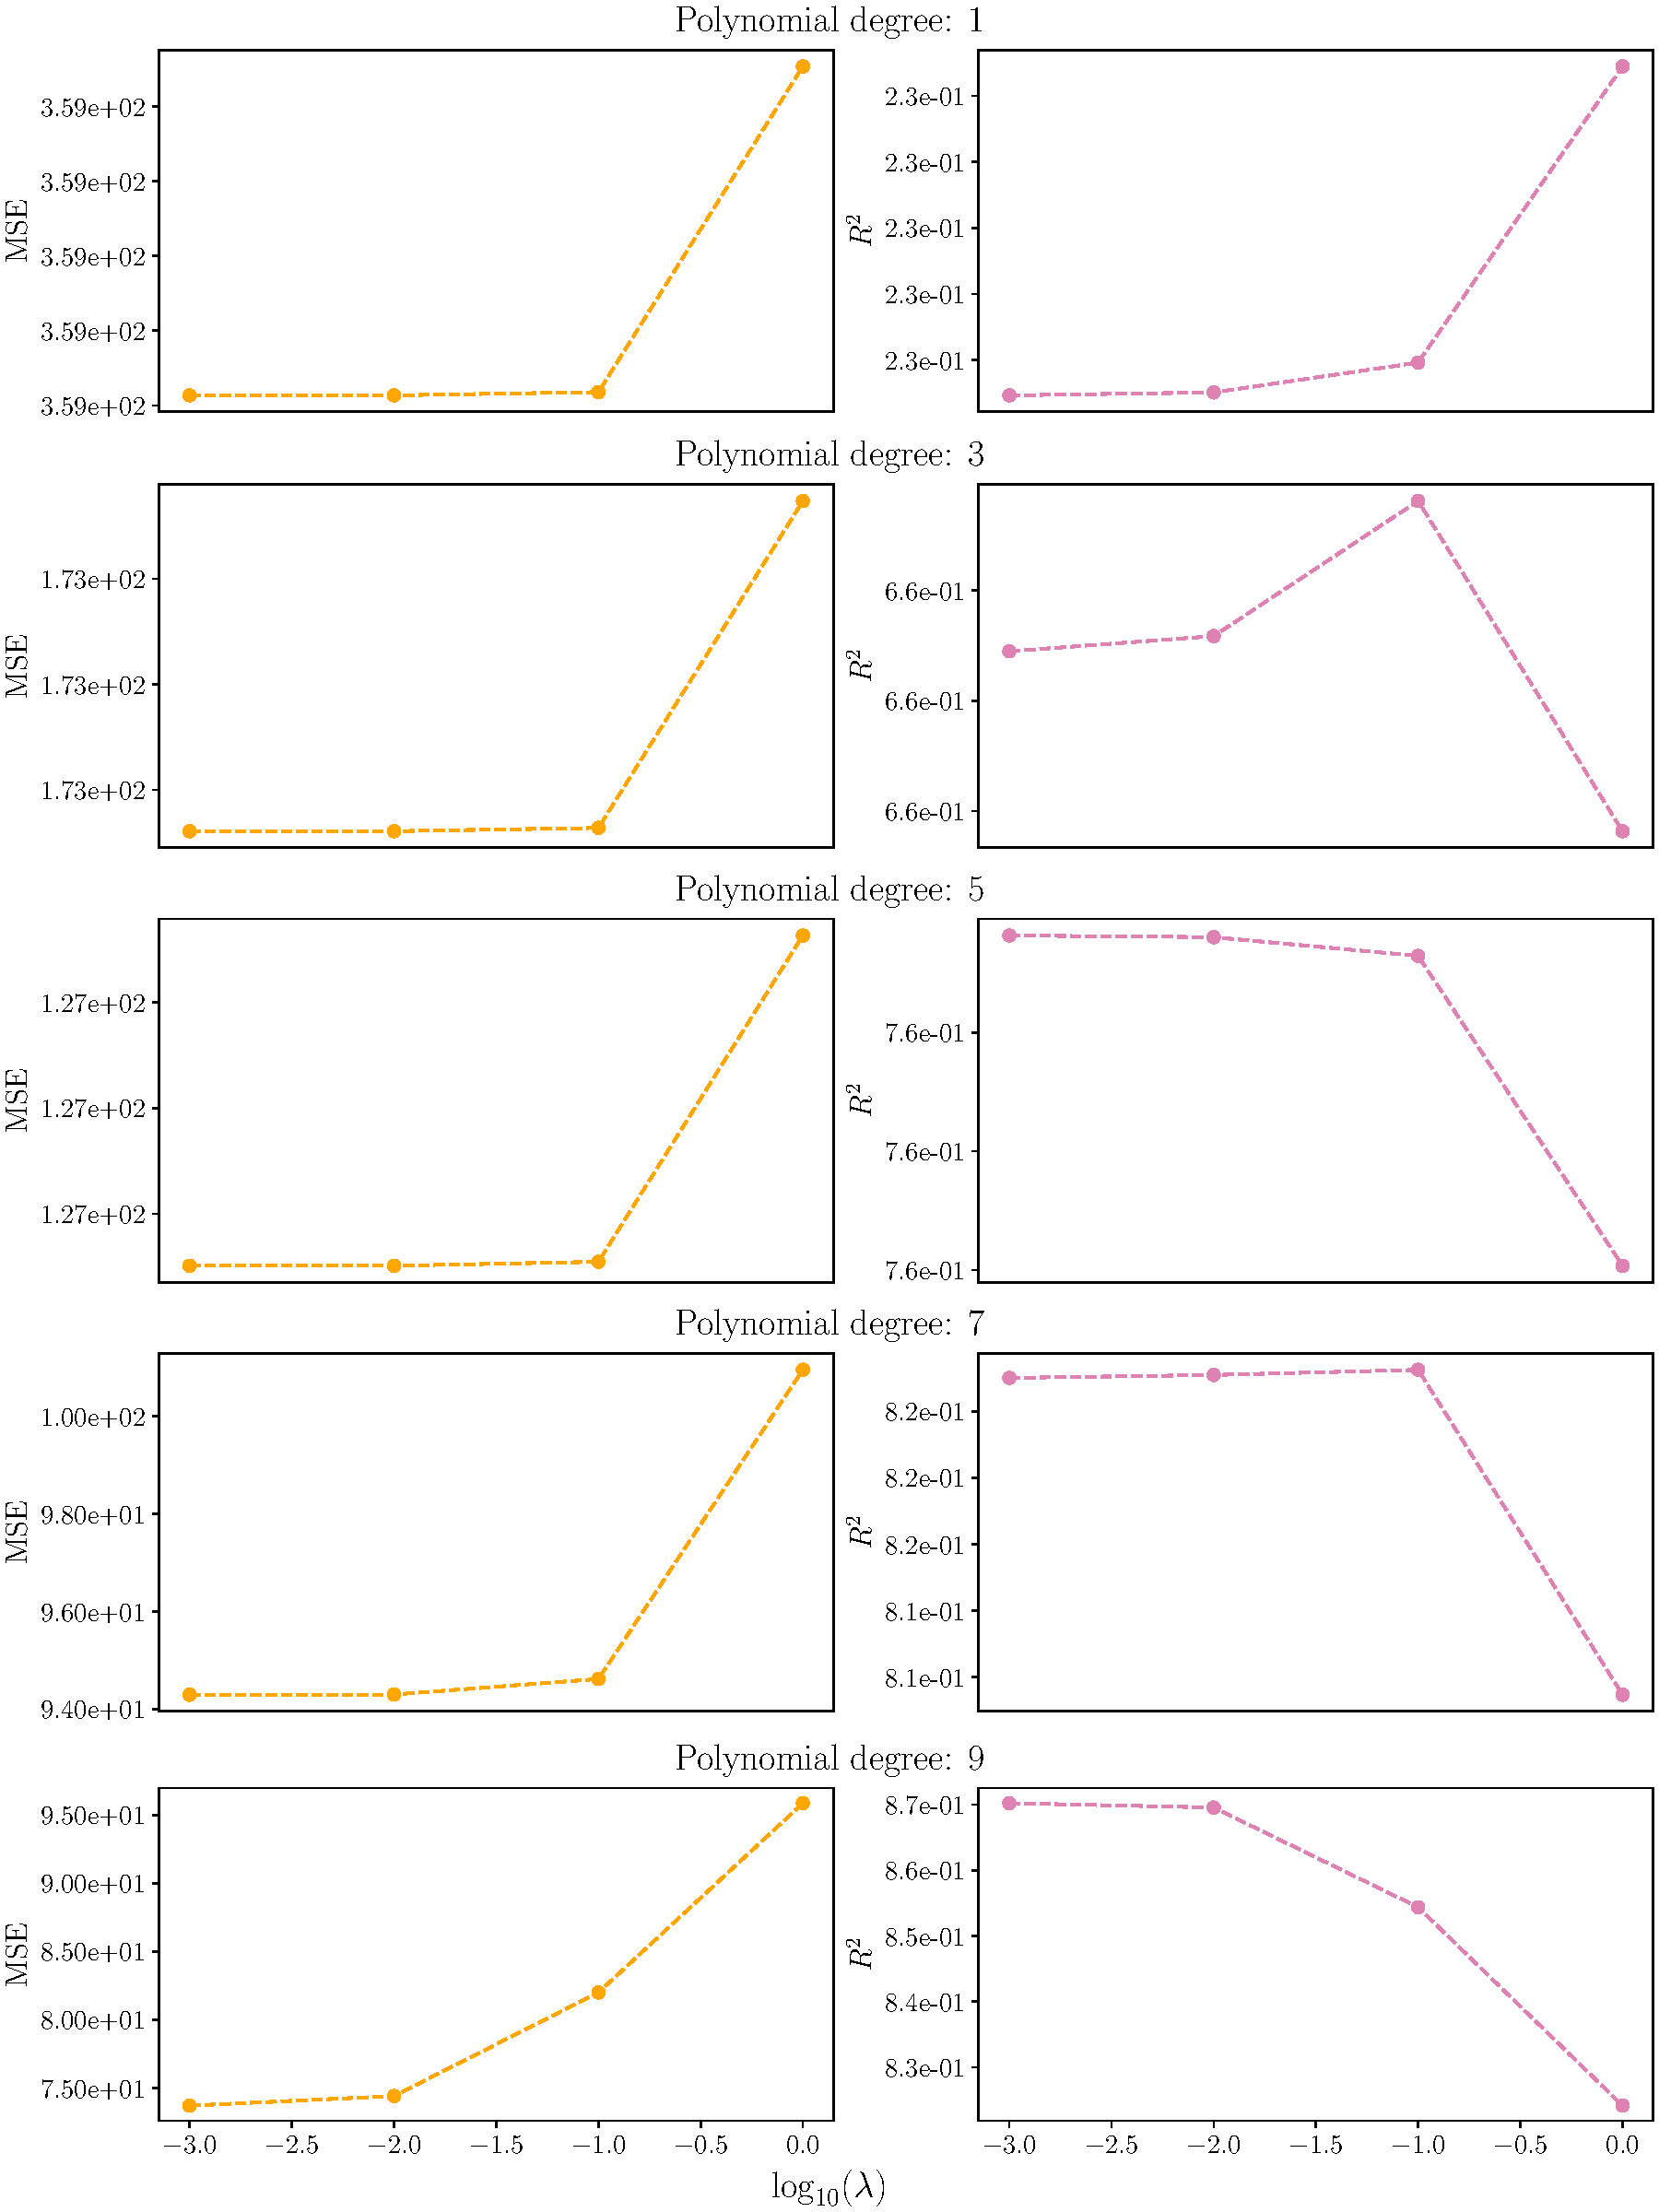
\includegraphics[trim = 0 0.75cm 0 0,clip,width=0.7\textwidth,keepaspectratio]{../figs/g_MSE_R2_Ridge.pdf}
%   \centering
%   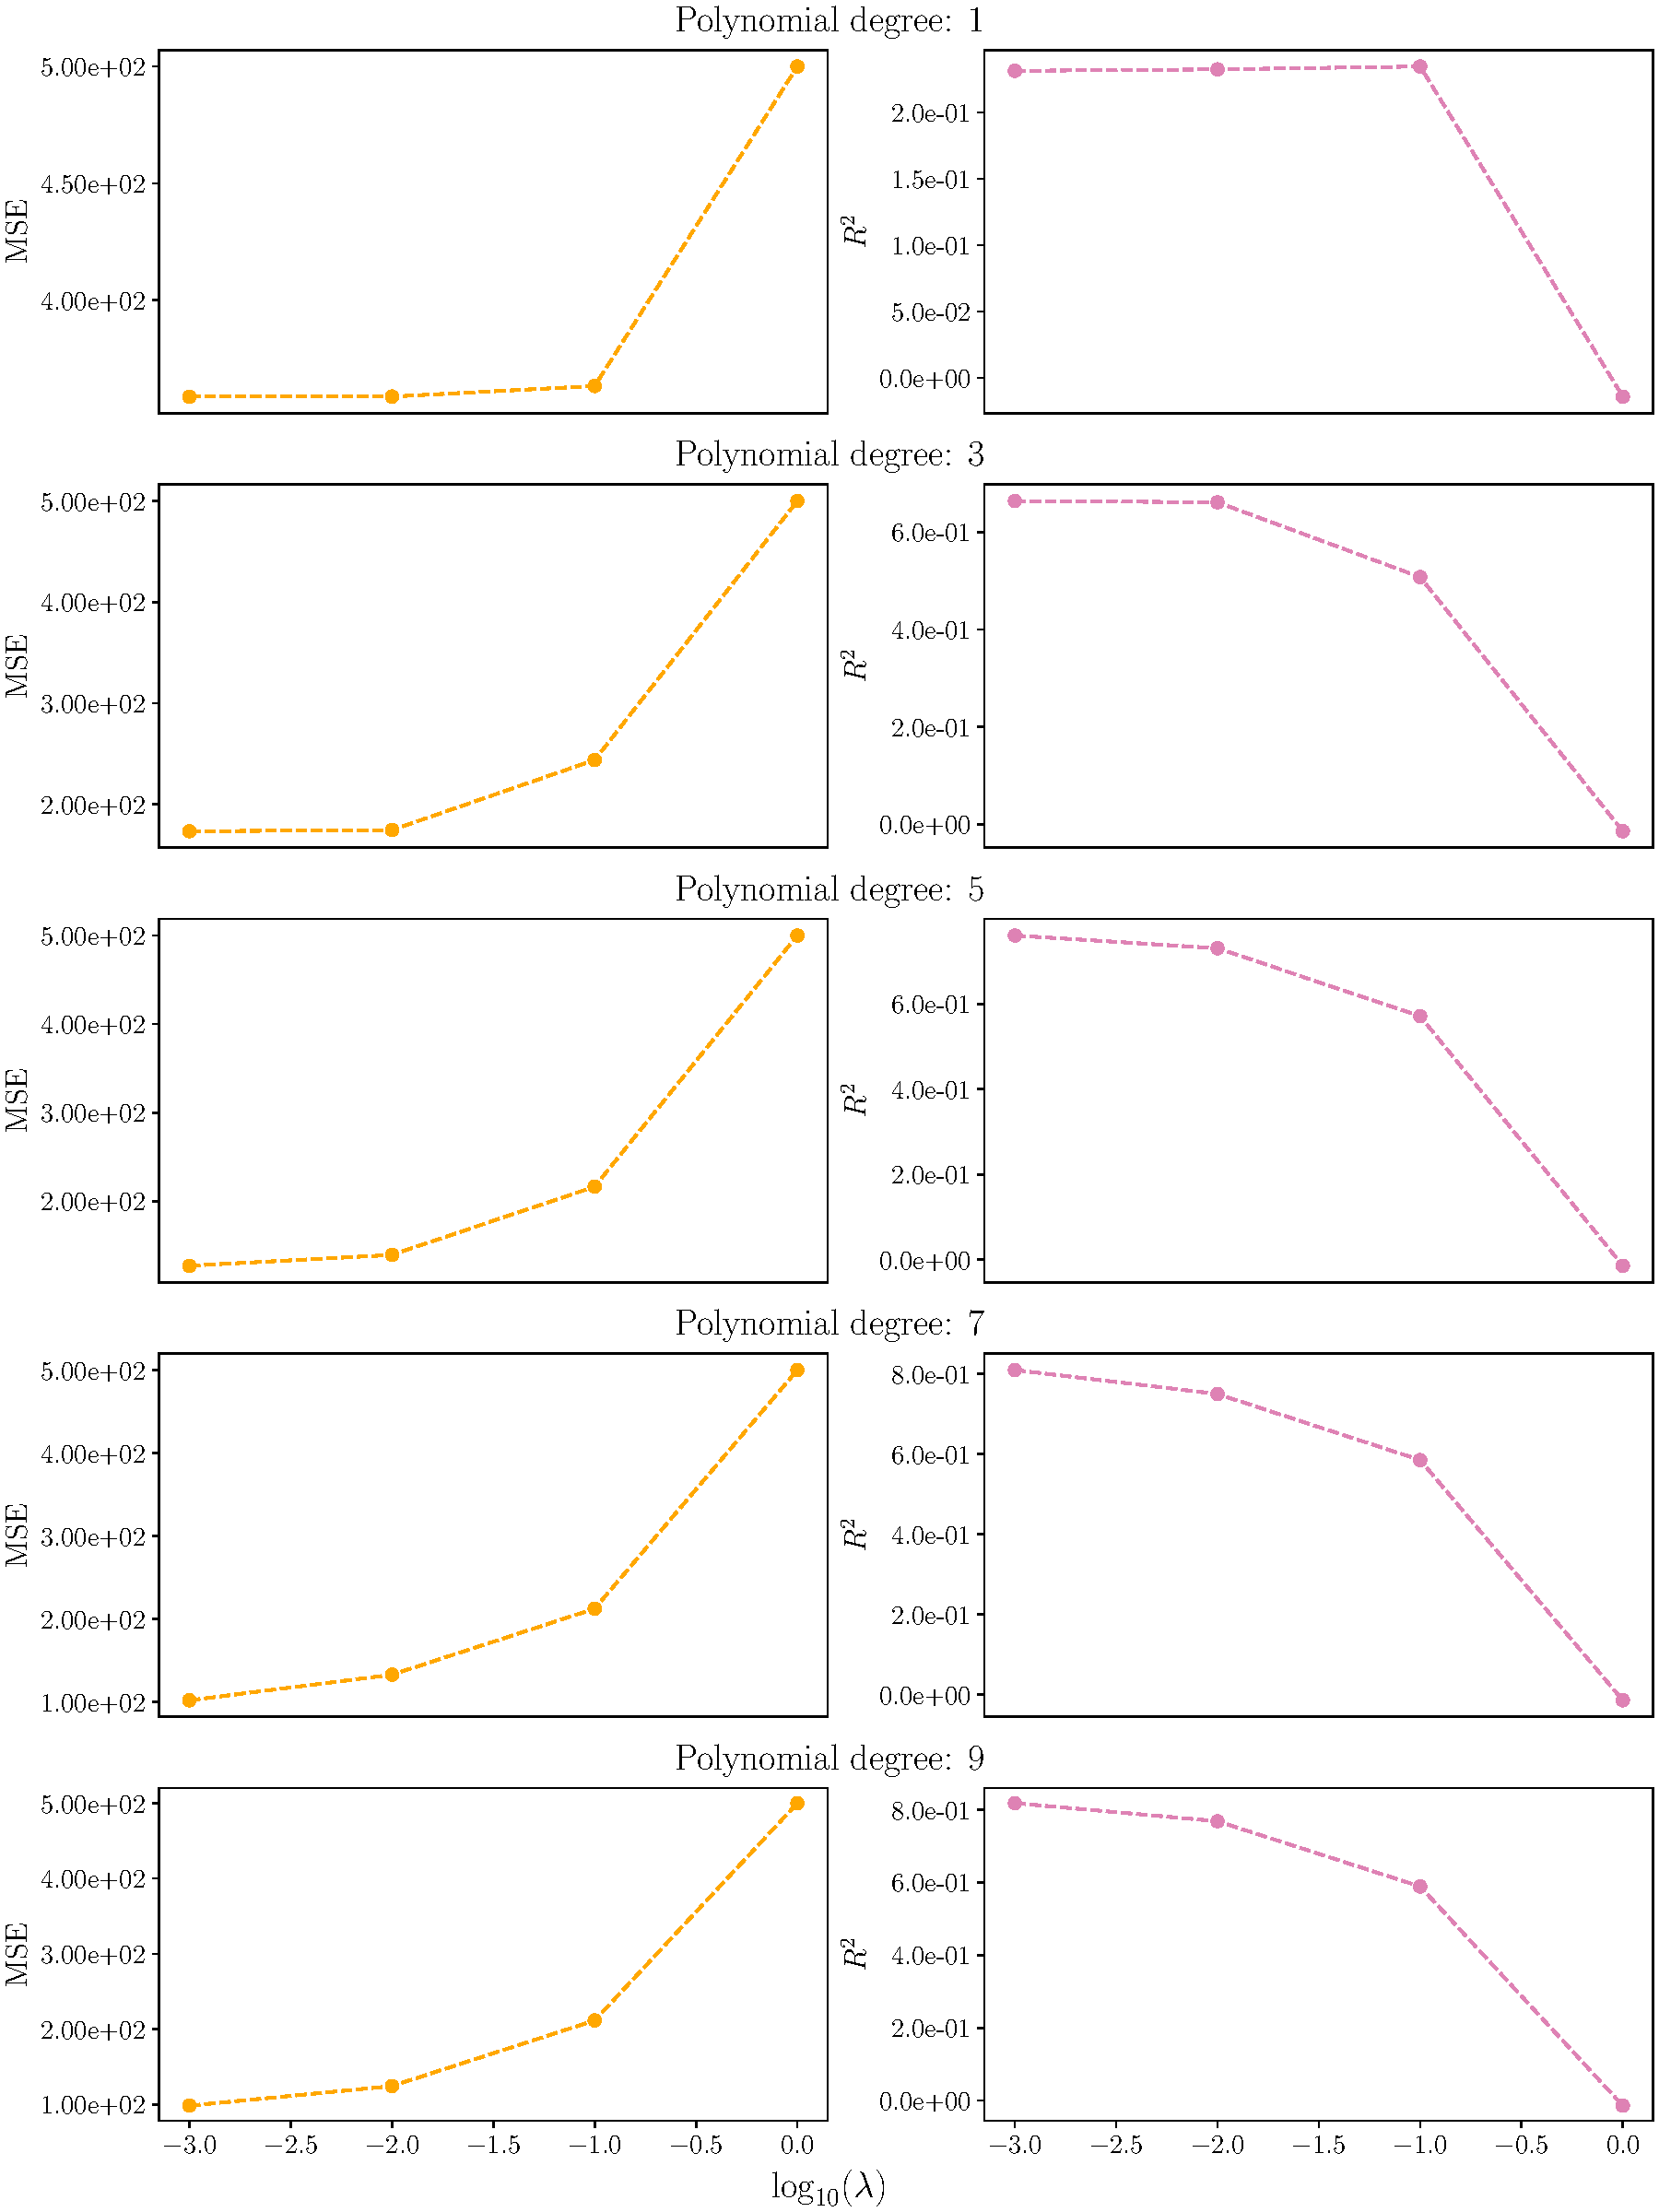
\includegraphics[width=0.7\textwidth]{../figs/g_MSE_R2_Lasso.pdf}
%   \caption{MSE (upper rows) and $R^2$ (lower rows) for Ridge (top section) and Lasso (bottom section) regression evaluated on the cosmological test set. The scores vary with polynomial degree horizontally and hyperparameter $\lambda$ vertically. In the right columns we have cropped away degrees smaller than 19, as well as the 3 largest $\lambda$'s only for Lasso, purely for visualization purposes.}\label{appfig:g MSE R2}
%   \vspace*{-5pt}
% \end{figure*}

\end{document}

% MAYBE REMOVE

% LINK WITH SPECIFIC NAME
% \href{https://raw.github.uio.no/oskarei/CompFys-Project5/main/data/gif/triple_slit_200_81_anim.gif?token=GHSAT0AAAAAAAAAIZKJAEIVBDMTTIDARGUYZMAXTHA}{triple-slit}

% MATHMODE IN HEADLINE
% \subsubsection{\texorpdfstring{$\text{Re}(u_{i,j}^n)$ and $\text{Im}(u_{i,j}^n)$}{Lg}}


% FIGURE COVERING BOTH COLUMNS
% \begin{figure*}
%   \vspace*{-5pt}
%   \centering %Centers the figure
%   \includegraphics[width=\textwidth]{../data/fig/triple_slit.pdf}
%   \caption{The square root of the probabilities at each point in the box $\sqrt{p_{i,j}^n}$ at the beginning (top left), middle (top center) and end (top right) of the triple-slit simulation with adjusted initialization and potential position. The plot at the bottom shows the normalized probability values $p(y\:|\:x=0.9;\;t=0.0025)$ along the detection screen at $x = 0.9$ at the end of the simulation.}\label{fig:TripleSlit}
%   \vspace*{-5pt}
% \end{figure*}

% FIGURE IN SINGLE COLUMN
% \begin{figure}[h!]
%   %\vspace*{-5pt}
%   \centering %Centers the figure
%   \includegraphics[width=0.9\columnwidth]{../data/fig/triple_sketch.png}
%   \caption{Illustration showing how the triple-slit interference pattern changes with distance from the slits. Gathered from Physics StackExchange \cite{TripleSketch}.}\label{fig:TripleSketch}
%   \vspace*{-10pt}
% \end{figure}


% TABLE COVERING BOTH COLUMNS
% \begin{center}
%   \vspace{-10pt}
%   \renewcommand{\arraystretch}{1.5}
%   \begin{table*}
%   %\centering
%   \begin{tabular}{| C{3.5cm} | C{2.2cm} | C{2.2cm} |  C{2.2cm} |  C{2.2cm} |  C{2.2cm} |  C{2.2cm} |}
%   \hline
%   \hspace{1pt} & \textbf{Model \hyperref[fig:potential model A]{A}} & \textbf{Model \hyperref[fig:potential model B]{B}} & \textbf{Model \hyperref[fig:potential model C]{C}} & \textbf{Model \hyperref[fig:potential model D]{D}} & \textbf{Model \hyperref[fig:potential model E]{E}} & \textbf{Model \hyperref[fig:potential model F]{F}} \\
%   \hline
%   \boldmath$m_0/M_{\astrosun}$ & $0.95$ & $0.95$ & $1.00$ & $1.00$ & $1.00$ & $1.05$ \\
%   \hline
%   \boldmath$r_0/R_{\astrosun}$ & $1.00$ & $1.25$ & $1.00$ & $1.00$ & $1.00$ & $1.50$ \\
%   \hline
%   \boldmath$L_0/L_{\astrosun}$ & $1.25$ & $1.00$ & $1.25$ & $1.50$ & $1.50$ & $1.00$ \\
%   \hline
%   \boldmath$\rho_0/\overline{\rho}_{\astrosun}$ & $1.00\times10^{-5}$ & $1.00\times10^{-5}$ & $7.50\times10^{-6}$ & $1.00\times10^{-5}$ & $2.50\times10^{-5}$ & $1.25\times10^{-5}$ \\
%   \hline
%   \textbf{Reach of }\boldmath{$m/m_0$} & $3.02\:\%$ & $4.24\:\%$ & $1.18\:\%$ & $2.66\:\%$ & $4.40\:\%$ & $3.79\:\%$ \\
%   \hline
%   \textbf{Reach of }\boldmath{$r/r_0$} & $0.73\:\%$ & $0.34\:\%$ & $0.06\:\%$ & $0.39\:\%$ & $0.51\:\%$ & $0.19\:\%$ \\
%   \hline
%   \textbf{Reach of }\boldmath{$L/L_0$} & $0.03\:\%$ & $0.14\:\%$ & $0.08\:\%$ & $0.04\:\%$ & $0.11\:\%$ & $0.21\:\%$ \\
%   \hline
%   \textbf{Size of core} & $0.24\times r_0$ & $0.19\times r_0$ & $0.26\times r_0$ & $0.25\times r_0$  & $0.24\times r_0$  & $0.15\times r_0$ \\
%   \hline
%   \textbf{Width of main zone} & $0.21\times r_0$ & $0.24\times r_0$ & $0.17\times r_0$ & $0.21\times r_0$ & $0.30\times r_0$ & $0.28\times r_0$ \\
%   \hline
%   \boldmath$F_\textbf{small}/F_\textbf{main}$ & No zone & No zone & $8.39\:\%$ & No zone & No zone & No zone \\
%   \hline
%   \end{tabular}
%   \cprotect\caption{The first four rows contain the initial mass, radius, luminosity and mass density of the six models, respectively. The initial temperature was $T_0 = 5770\:\text{K}$ for all six models, and the initial pressure was decided by the initial mass density through the equation of state. The next three rows show how far $m$, $r$ and $L$ reached before the integration was stopped, respectively. The size of the core and of the main convection zone near the surface, both given in units of $r_0$, are listed in the two next rows. In the last row I have listed the ratios between the convective flux from an eventual second, smaller convection zone and the convective flux from the respective main convection zone. If it says ``No zone'', the model does not have any more convection zones.}\label{tab:models}
%   \end{table*}
%   \renewcommand{\arraystretch}{1}
%   \vspace{-20pt}
% \end{center}

% STANDARD TABLE IN SINGLE COLUMN
% \begin{center}
%   \renewcommand{\arraystretch}{1.5}
%   \begin{table}[h!]
%   \centering
%   \begin{tabular}{| C{2.2cm} | C{1.4cm} | C{1.4cm} | C{1.4cm} | C{1.4cm} |}
%   \hline
%   \textbf{No. of cycles} & \boldmath$\left<ϵ\right>$ \boldmath$[J]$ & \boldmath$\left<|m|\right>$ & \boldmath$C_V$ \boldmath$[k_\text{B}]$ & \boldmath$\chi$ \boldmath$[J^{-1}]$ \\
%   \hline
%   10 & $-1.8000$ & 0.9375 & 1.4400 & 0.1594 \\
%   \hline
%   20 & $-1.9000$ & 0.9688 & 0.7600 & 0.0836 \\
%   \hline
%   50 & $-1.9600$ & 0.9875 & 0.3136 & 0.0344 \\
%   \hline
%   100 & $-1.9800$ & 0.9938 & 0.1584 & 0.0173 \\
%   \hline
%   200 & $-1.9775$ & 0.9931 & 0.1780 & 0.0186 \\
%   \hline
%   500 & $-1.9880$ & 0.9962 & 0.0954 & 0.0104 \\
%   \hline
%   1000 & $-1.9940$ & 0.9981 & 0.0479 & 0.0052 \\
%   \hline
%   5000 & $-1.9960$ & 0.9988 & 0.0319 & 0.0033 \\
%   \hline
%   10000 & $-1.9974$ & 0.9992 & 0.0204 & 0.0022 \\
%   \hline
%   100000 & $-1.9975$ & 0.9992 & 0.0197 & 0.0022 \\
%   \hline
%   1000000 & $-1.9973$ & 0.9992 & 0.0215 & 0.0023 \\
%   \hline
%   \textbf{Analytical} & $-1.9960$ & 0.9987 & 0.0321 & 0.0040 \\
%   \hline
%   \end{tabular}
%   \cprotect\caption{Numerical estimates of $\left<\epsilon\right>$, $\left<|m|\right>$, $C_V$ and $\chi$ for $T = 1.0\:J/k_\text{B}$ after increasing numbers of Monte Carlo cycles are performed. The last row contains the analytical values.}\label{tab:2x2 results}
%   \end{table}
%   \renewcommand{\arraystretch}{1}
% \end{center}

% TABLE WITH MULTIROW
% \begin{center}
%   \renewcommand{\arraystretch}{1.5}
%   \begin{table}[h!]
%   \centering
%   \begin{tabular}{| C{2.4cm} | C{1.5cm} | C{1.1cm} | C{2.0cm} |}
%   \hline
%   \textbf{No. of} \boldmath$s = +1$ & \boldmath$E(\mathbf{s})$ \boldmath$[J]$ & \boldmath$M(\mathbf{s})$ & \textbf{Degeneracy} \\
%   \hline
%   0 & $-8$ & $-4$ & None \\
%   \hline
%   1 & \hspace{7pt}$0$ & $-2$ & $4$ \\
%   \hline
%   \multirow{2}{*}{2} & \hspace{7pt}$8$ & \multirow{2}{*}{\hspace{7pt}$0$} & $2$ \\
%   \cline{2-2}\cline{4-4}
%   & \hspace{7pt}$0$ & & $4$ \\
%   \hline
%   3 & \hspace{7pt}$0$ & \hspace{7pt}$2$ & $4$ \\
%   \hline
%   4 & $-8$ & \hspace{7pt}$4$ & None \\
%   \hline
%   \end{tabular}
%   \cprotect\caption{Total energy $E(\mathbf{s})$ and magnetisation $M(\mathbf{s})$ for a \texorpdfstring{$2\times2$}{Lg} lattice with $0$, $1$, $2$, $3$ and $4$ spins $s = +1$. Because we use periodic boundary conditions, the total energy can either be 0$\:J$ or 8$\:J$ when we have two spins $s = +1$ and two spins $s = -1$, depending on if the equal spins are neighbours or not. The last column contains the degeneracy level for the different combinations of number of spins $s = +1$ and total energy.}\label{tab:2x2 lattice}
%   \end{table}
%   \renewcommand{\arraystretch}{1}
% \end{center}


% ALGORITHM
% \begin{figure}
%   % NOTE: We only need \begin{figure} ... \end{figure} here because of a compatability issue between the 'revtex4-1' document class and the 'algorithm' environment.
%       \begin{algorithm}[H]
%       \caption{The Metropolis Algorithm}
%       \label{algo:Euler}
%           \begin{algorithmic}
%               \Procedure{Monte Carlo cycle}{$\mathbf{s}, L, β$}
%               \For{$i = 0, 1, \ldots, L-1$}
%               \For{$j = 0, 1, \ldots, L-1$}
%               \State $\triangleright$ Compute energy difference due to flipping $s_{ij}$
%               \State $\Delta E ← \Delta E_\text{function}(\mathbf{s}, i, j)$
%               \State
%               \State $\triangleright$ Flip if energy difference is negative or zero
%               \If{$\Delta E \leq 0$}
%                   \State $s_{ij} = -s_{ij}$ \Comment{Flip spin}
%                   \State
%               \Else \Comment{Energy difference is positive}
%                   \State $w = e^{-β\Delta E}$ \Comment{Probability of flipping spin}
%                   \State $\triangleright$ Generate random number $r ∈ [0,1]$
%                   \State $\triangleright$ Flip spin if $r≤ w$
%                   \If{$r≤ w$}
%                       \State $s_{ij} = -s_{ij}$ \Comment{Flip spin}
%                   \EndIf
%               \EndIf
%               \State 
%               \State $\triangleright$ Calculate $E$, $E^2$, $|M|$ and $M^2$ for $\mathbf{s}$
%               \State $E$, $E^2 = E_\text{function}(\mathbf{s})$
%               \State $|M|$, $M^2 = M_\text{function}(\mathbf{s})$
%               \State $\triangleright$ Update expectation values accordingly
%               \EndFor
%               \EndFor
%               \EndProcedure
%           \end{algorithmic}
%       \end{algorithm}
%   \end{figure}